%% Manuscript — Interlocked Credit in Bangladesh Rice Markets
%% Formatted with elsarticle (World Development style); not submitted to any journal.
%% Compile: pdflatex main && bibtex main && pdflatex main && pdflatex main
%% Or:       latexmk -pdf main
%%
%% Document class options (following elsarticle-template-harv.tex):
%%   preprint    -- single-column draft layout
%%   review      -- adds double line spacing for peer review
%%   authoryear  -- natbib author-year citations
%%   12pt        -- submission font size

\documentclass[authoryear,preprint,review,12pt]{elsarticle}

%% elsarticle prints "Preprint submitted to <journal>" on page 1; this is a
%% working paper, so replace that footer.
\makeatletter
\def\ps@pprintTitle{%
  \let\@oddhead\@empty
  \let\@evenhead\@empty
  \def\@oddfoot{\footnotesize\itshape Working paper\hfill November 2026}%
  \let\@evenfoot\@oddfoot}
\makeatother

%% ── Encoding & fonts ─────────────────────────────────────────────────────────
\usepackage{lmodern}
\usepackage[T1]{fontenc}
\usepackage[utf8]{inputenc}
\usepackage[protrusion=true,expansion=false]{microtype}

%% ── Tables ───────────────────────────────────────────────────────────────────
\usepackage{booktabs}
\usepackage{siunitx}
\sisetup{
  table-number-alignment = center,
  table-figures-decimal  = 3,
  table-space-text-post  = ***,
  detect-all
}
\usepackage{threeparttable}
\usepackage{array}
\usepackage{multirow}
\usepackage{longtable}

%% ── Figures ──────────────────────────────────────────────────────────────────
\usepackage{graphicx}

%% ── Math ─────────────────────────────────────────────────────────────────────
\usepackage{amsmath}
\usepackage{amssymb}

%% ── Layout ───────────────────────────────────────────────────────────────────
\usepackage{lineno}
\usepackage{setspace}
\usepackage[margin=1in]{geometry}
\usepackage{hyperref}
\hypersetup{colorlinks=true, linkcolor=blue, citecolor=blue, urlcolor=blue}

%% ── Custom commands ──────────────────────────────────────────────────────────
\newcommand{\sym}[1]{\ensuremath{^{#1}}}
\newcommand{\BDT}{BDT}
\newcommand{\citea}[1]{\citeauthor{#1} (\citeyear{#1})}

%% ─────────────────────────────────────────────────────────────────────────────
\begin{document}

\linenumbers

\begin{frontmatter}

\title{Interlocked Credit in Agricultural Commodity Markets:\\
       Prevalence, Structure, and Market Implications\\
       in Bangladesh's Rice Trading Sector}

\author[ifpri]{Razin Kabir\corref{cor1}}
\ead{R.Kabir@cgiar.org}

\cortext[cor1]{Corresponding author.}
\affiliation[ifpri]{organization={International Food Policy Research Institute (IFPRI)},
             city={Washington, DC},
             country={USA}}

\begin{abstract}
Interlocked credit---the tying of supplier credit to commodity procurement
relationships---is a defining feature of agricultural markets in developing
countries, yet its prevalence and market implications remain poorly documented
outside Sub-Saharan Africa. Using the 2018 Bangladesh Millers and Traders
Survey (866 traders, 36 districts), we provide the first nationally representative
characterisation of interlocked credit in Bangladesh's rice
trading sector. Credit is near-universal: 82~percent of paddy trader-season
observations involve supplier credit, with substantial variation by trader
type, season, and geography. Despite this pervasiveness, regression analysis
finds no significant within-market price discount associated with credit
receipt---a result robust to instrumental variable estimation. The dominant
form of credit appears to operate as relationship capital rather than as an
instrument of price manipulation: 94.5~percent of credit-holding traders
report no explicit price premium, while the minority who do face implied
annual rates of 51~percent---consistent with a thin, high-rate residual
segment. Credit is also associated with \emph{higher}, not lower,
within-season price variance, suggesting that credit enables access to
a broader range of market conditions rather than smoothing liquidity
constraints. These findings have implications for policy interventions
targeting credit access and market competition in agricultural supply chains.
\end{abstract}

%%Research highlights
\begin{highlights}
\item First large-scale national survey evidence on interlocked credit in Bangladesh rice trade
\item Supplier credit is near-universal: 82\% of paddy trader-seasons involve credit
\item No significant within-market price discount from credit (OLS and IV)
\item Explicit price premium reporters face implied annual rates of 51\% (median)
\item Credit associated with higher within-season price variance, not lower
\end{highlights}

\begin{keyword}
interlocked markets \sep credit markets \sep commodity trade \sep Bangladesh
\sep rice \sep agricultural finance \sep market structure \\[3pt]
\textit{JEL Classification:} Q13 \sep Q14 \sep O13 \sep L14 \sep G21
\end{keyword}

\end{frontmatter}

%% ─────────────────────────────────────────────────────────────────────────────
\section{Introduction}
\label{sec:intro}

Agricultural commodity markets in developing countries are characterised
by the simultaneous exchange of credit and commodities. Suppliers extend
credit to buyers; buyers advance payments to farmers; commission agents
enforce repayment through ongoing trade relationships. This interlinking
of factor and product markets---what \citet{bardhan1980} called
``interlinked transactions''---has been theorised to generate welfare costs
for smallholder farmers by depressing procurement prices below competitive
levels as a form of implicit interest \citep{braverman_stiglitz1982}.
The stakes are potentially large: in countries where paddy farming provides
livelihoods for a significant share of the rural workforce, procurement
price wedges of even a few percentage points can account for a meaningful
fraction of smallholder income, representing a transfer from producers to
buyers that is invisible to standard market monitoring instruments.

Despite four decades of theoretical development, rigorous empirical evidence
on interlocked credit in agricultural markets remains sparse, particularly
for South Asia. The limited evidence that exists is concentrated in
Sub-Saharan Africa \citep{fafchamps_minten1999, stephens_barrett2011},
where survey-based studies document credit prevalence of 30--60~percent
among grain traders but rarely observe the transaction-level price data
needed to directly test for price suppression. Foundational work on South
Asian agricultural credit \citep{murshid1992, crow_murshid1994} relied on
qualitative case studies that, while analytically rich, cannot speak to
national prevalence or estimate market-level price effects at scale. The
specific Bangladesh context has been revisited \citep{murshid2015}, but
without the representative quantitative data needed to assess whether
historical interlocking patterns have persisted or transformed.

This paper fills this gap using the 2018 Bangladesh Millers and Traders
Survey (MATS), a large national survey covering 798 millers and 866 traders
across all eight divisions of Bangladesh \citep{dorosh_etal2021}. The miller
component was designed as a two-stage stratified probability sample and is
nationally representative; the trader component was constructed via a snowball
approach in which sampled millers identified their most important buyers and
suppliers, yielding broad geographic coverage (36 districts) but a sample
likely over-representing traders who deal directly with millers rather than
terminal traders. The survey's detailed Module D asks traders directly about
credit arrangement types, payment mode composition, credit duration, and
monthly procurement prices---variables that map precisely onto the theoretical
constructs of interlocked credit and enable, for the first time, a large-scale
nationally distributed characterisation of these arrangements in a major South
Asian agricultural market.

Bangladesh is an important setting for three reasons. First, rice is the
primary staple and the dominant agricultural commodity, with annual paddy
production exceeding 50 million metric tons and a complex multi-tier trading
structure that is emblematic of South Asian grain markets more broadly.
Second, Bangladesh has undergone rapid financial inclusion since 2010 through
bKash and other mobile money platforms---making it possible to ask whether
credit interlocking persists even as formal and digital payment options expand.
Third, the MATS survey was specifically designed to capture credit arrangements,
providing variable quality that most general agricultural surveys lack.

The null result itself carries information beyond the failure to confirm
Braverman-Stiglitz. A growing body of theory and evidence argues that the
welfare costs of interlocked credit operate primarily through mechanisms
other than observable price wedges---lock-in to a credit-extended buyer
limits effective competition even when many buyers are present
\citep{crow_murshid1994}, and relationship rents may be captured through
non-price margins (supply certainty, priority access, quality enforcement)
rather than through explicit price differences \citep{casaburi_macchiavello2019}.
Our findings are consistent with this relational contracting interpretation:
credit is near-universal, persistent alongside mobile money, and associated
with higher price variance rather than lower prices, suggesting it operates
as a market-access and relationship-capital institution rather than a
price-manipulation instrument. This shifts the policy question from ``are
prices being depressed?'' to ``who is locked in and who bears the cost of
exit?''---a question that requires different data and different interventions.

Our analysis makes three contributions. First, we document that interlocked
credit is far more pervasive in Bangladesh than in the African markets most
studied in the literature: 82~percent of paddy trader-season observations
involve supplier credit (Table~\ref{tab:comparison}), exceeding rates of
30--60~percent documented in Sub-Saharan Africa. This prevalence is not
uniform---it varies substantially by trader type (aratdars more than
faria/bepari), season (the minor Aus season is an outlier with near-universal
all-supplier credit), and geography (from 100~percent in several eastern
districts to below 35~percent in coastal Barisal).

Second, we show that credit is overwhelmingly implicit in its pricing:
94.5~percent of credit-holding traders report no explicit price premium for
buying on credit. Among the 5.5~percent who do, the implied annual interest
rate is 51~percent at the median---far above formal bank lending rates but
within the range of informal credit in South Asian agriculture. This dual
structure---near-universal implicit credit alongside a thin, explicitly priced
residual segment---is consistent with models of relational contracting
\citep{hoff_stiglitz1990, casaburi_macchiavello2019} in which most credit
serves as relationship capital rather than surplus extraction.

Third, we test the central prediction of \citet{braverman_stiglitz1982}---that
interlocked credit depresses procurement prices---and find no supporting
evidence within local markets. OLS regressions with upazila, season, and
month fixed effects and IV estimates using leave-one-out credit rates both
yield small, insignificant price coefficients. A key structural reason is
that more than 60~percent of upazila-season market cells have \emph{all}
surveyed traders using credit: within-market variation in credit status
is largely absent, meaning price-based interlocking of the Braverman-Stiglitz
type simply cannot operate at this level of aggregation. Credit's competitive
effects appear to operate instead through lock-in and relationship rents
rather than observable price wedges, with implications for how policymakers
should think about credit access and market competition.

The remainder of the paper is structured as follows. Section~\ref{sec:theory}
reviews the theoretical framework and existing evidence. Section~\ref{sec:data}
describes the data and context. Section~\ref{sec:descriptive} presents the
descriptive evidence on credit structure. Section~\ref{sec:determinants}
analyses the correlates of credit use. Section~\ref{sec:prices} tests the
price effect. Section~\ref{sec:implications} discusses market structure
implications and policy relevance. Section~\ref{sec:conclusion} concludes.

%% ─────────────────────────────────────────────────────────────────────────────
\section{Theoretical Framework and Existing Evidence}
\label{sec:theory}

\subsection{Interlocked Credit and Price Effects}

Interlocked transactions arise when two or more markets---here, credit and
commodity trade---are linked in a single contractual arrangement
\citep{bardhan1980}. The theoretical interest in interlinked markets stems
from the observation that each market's imperfections can compound when they
are tied together: a buyer who is also a lender faces a combined optimization
problem in which credit terms and commodity prices are jointly determined, and
the resulting contract can exploit the seller's vulnerability across both
dimensions simultaneously. In agricultural settings, the prototypical form
is a commodity buyer who simultaneously extends credit to a farmer or upstream
trader, with repayment in the form of commodity delivery at a price potentially
below the competitive market rate.

\citet{braverman_stiglitz1982} formalise this mechanism, showing that a
monopsonistic buyer can exploit the credit channel to extract surplus from a
credit-constrained supplier: the credit is ``priced'' through a below-market
procurement price rather than an explicit interest rate, making the transaction
harder to identify and regulate. The mechanism requires two conditions. First,
the seller must face a binding credit constraint and be unable to obtain
working capital at competitive rates outside the bilateral relationship.
Second, the buyer must possess sufficient market power that the seller cannot
costlessly exit to find an alternative buyer on better terms. Under these
conditions, the buyer can decompose a below-market procurement price into an
implicit interest component and a competitive-price component, with the
interest payment camouflaged within the commodity transaction. \citet{bell1988}
provides a comprehensive review of this class of models, showing that
interlocking is a rational response to the co-existence of thin credit markets
and imperfect commodity market competition.

The welfare predictions of this model are stark: interlocked credit depresses
farm-gate prices, transfers surplus from producers to buyers, and can lock
farmers and small traders into bilateral relationships that reduce their
effective market access---even when many buyers are physically present
\citep{crow_murshid1992}. \citet{ray_sengupta1989} show that surplus extraction
can also operate through the quantity of credit offered: a monopsonistic buyer
may deliberately restrict credit supply in ways that limit the seller's ability
to diversify marketing relationships, amplifying lock-in effects. Empirical
tests of these predictions require data on both credit arrangements and prices
within the same market, which is rarely available from standard agricultural
surveys.

\subsection{Competitive Equilibrium and Relational Contracting Alternatives}

The Braverman-Stiglitz prediction rests on monopsonistic or oligopsonistic
market power. If credit markets are locally competitive---if many buyers offer
credit on similar terms---the mechanism cannot generate price wedges: sellers
who perceive unfavourable implicit pricing can credibly threaten to move to
a competing buyer, disciplining contract terms. In this competitive equilibrium,
credit becomes a standard feature of market participation rather than an
instrument of surplus extraction, and near-universal credit prevalence is
itself consistent with a competitive rather than exploitative outcome.
\citet{hoff_stiglitz1990} show that even informal credit markets can be
locally competitive, with credit rates reflecting information rents and
enforcement costs rather than monopoly power. Critically, widespread credit
use can be evidence of competition rather than exploitation: if buyers must
offer credit to attract suppliers, entry-level universality of credit is
the long-run competitive equilibrium outcome.

A second mechanism is financial deepening: as sellers gain access to formal
or semi-formal credit---through microfinance institutions, mobile money, or
MSME lending---they can substitute independent financing for buyer credit,
reducing the hold of bilateral relationships \citep{conning_udry2007,
karlan_etal2014}. This predicts that credit interlocking should be more
prevalent among financially excluded sellers and should decline with
financial inclusion. The persistence of interlocked credit in Bangladesh
despite the rapid growth of bKash and other mobile money platforms would,
under this view, indicate that these products have not yet substituted for
trade credit functions---a testable implication we examine in the determinants
analysis.

A third and substantively distinct alternative is the relational contracting
interpretation \citep{casaburi_macchiavello2019, blouin_macchiavello2019}:
credit embedded in ongoing buyer-supplier relationships functions primarily
as a commitment and enforcement device, providing guaranteed supply and
quality assurance to the buyer and working capital to the seller. In markets
where commodity quality is difficult to verify before purchase, delivery
commitments are hard to enforce, or post-harvest trading is seasonal and
intermittent, bilateral credit relationships can sustain cooperation on
non-price dimensions that anonymous spot markets cannot support. Under this
interpretation, the ``rent'' captured through credit relationships is embodied
in supply certainty and reduced search costs rather than in a below-market
procurement price---and the relationship may be welfare-improving for both
parties relative to spot market trading. \citet{casaburi_macchiavello2019}
provide the most direct empirical test in a developing country agricultural
context, finding in Kenyan dairy supply chains that infrequent-payment
arrangements serve as commitment devices enabling farmers to accumulate
precautionary savings---rather than as instruments of price manipulation. This interpretation predicts
near-zero explicit price effects but potentially significant effects on
supply security, market access, and relationship stability.

\subsection{Evidence from Other Agricultural Markets}

Table~\ref{tab:comparison} places Bangladesh in comparative context.
A small but growing empirical literature documents credit prevalence in
agricultural commodity trade across developing countries, concentrated
in Sub-Saharan Africa.

\citet{fafchamps_minten1999} document that 35--55~percent of grain traders
in Madagascar use supplier credit, with credit concentrated among
larger-volume traders who have established long-term supplier relationships.
Their work on the institutional foundations of agricultural trade emphasises
that relationship-based credit substitutes for weak contract enforcement
and property rights---a different function from the price-suppression
mechanism but equally central to understanding why credit interlocking
persists. \citet{fafchamps_minten2002} further show that social network
capital among Madagascar traders raises productivity without systematically
enabling anti-competitive pricing, underscoring the complex relationship
between credit networks and market competition. \citet{stephens_barrett2011}
document 30--60~percent credit use among maize traders in Kenya and find
that credit-using traders access a broader range of markets and sources,
consistent with credit facilitating rather than restricting market
participation. \citet{barrett2008} reviews the broader evidence on
smallholder market participation in Africa, showing that liquidity
constraints at harvest force distress sales at below-market prices---a
mechanism that parallels the B-S prediction even in the absence of
explicit credit interlocking.

The most rigorous and methodologically closest study is \citet{casaburi_macchiavello2019},
who exploit the institutional structure of Kenyan tea buying stations to
show that infrequent-payment arrangements---a form of delayed settlement
that creates buyer credit from the farmer's perspective---serve primarily
as commitment devices enabling farmers to accumulate precautionary savings.
Their findings explicitly support the relational contracting over the
price-suppression interpretation. \citet{blouin_macchiavello2019} provide
complementary evidence from international coffee markets, showing that
relationship capital shapes default patterns in ways consistent with
long-term rents being sustained through supply reliability rather than
price wedges.

South Asian evidence is substantially thinner. The foundational work by
\citet{murshid1992} and \citet{crow_murshid1992} documents, through detailed
case studies of Bangladesh rice and wheat markets, that credit interlocking
was pervasive in the early 1990s and that mechanisms resembling Braverman-Stiglitz
price suppression were qualitatively present. \citet{crow_murshid1992}
describe a pattern of ``vertical interlocking''---credit flowing across
stages of the supply chain in ways that restricted seller mobility even
when multiple buyers were physically accessible. However, these studies
cannot quantify prevalence, estimate causal price effects, or assess
whether findings reflect systemic patterns or specific market configurations.
The present paper provides the first large-scale quantitative evidence on
these questions for a major South Asian grain market.

\begin{table}[tp]
  \centering
  \caption{Interlocked Credit in Agricultural Markets: Comparative Evidence}
  \label{tab:comparison}
  \begin{singlespace}
  \small
  \begin{threeparttable}
    \begin{tabular}{>{\raggedright\arraybackslash}p{4.2cm}>{\raggedright\arraybackslash}p{2.8cm}>{\raggedright\arraybackslash}p{1.6cm}>{\raggedright\arraybackslash}p{2.2cm}>{\raggedright\arraybackslash}p{2.5cm}}
\toprule
Study & Country/market & Credit prev. & Explicit pricing & Data type \\
\midrule
\multicolumn{5}{l}{\textit{Sub-Saharan Africa}} \\
\addlinespace[2pt]
\citet{fafchamps_minten1999} & Madagascar grain & 35--55\% & Not reported & Trader survey \\
\citet{stephens_barrett2011} & Kenya maize & 30--60\% & Rare & Panel \\
\citet{casaburi_macchiavello2019} & Kenya dairy & High & Implicit & Admin panel \\
\addlinespace[4pt]
\multicolumn{5}{l}{\textit{South Asia}} \\
\addlinespace[2pt]
\citet{murshid1992} & Bangladesh rice & Not rep. & Not quantified & Case studies \\
\citet{crow_murshid1992} & Bangladesh rice & Not rep. & Not quantified & Case studies \\
\textbf{This study} & \textbf{Bangladesh rice} & \textbf{82\%} & \textbf{5.5\% explicit} & \textbf{Large-scale survey} \\
\bottomrule
\end{tabular}

    \begin{tablenotes}\footnotesize
      \item \textit{Notes:} Selected studies documenting interlocked credit
      in agricultural commodity markets. Credit prevalence figures are for
      the most comparable arrangement measure available in each study.
    \end{tablenotes}
  \end{threeparttable}
  \end{singlespace}
\end{table}

%% ─────────────────────────────────────────────────────────────────────────────
\section{Context and Data}
\label{sec:data}

\subsection{Bangladesh's Rice Trading Structure}

Rice is Bangladesh's primary staple crop and the dominant agricultural
commodity, with annual paddy production exceeding 50 million metric tons
across three distinct growing seasons: the main Aman (wet-season, harvested
November--January), the irrigated Boro (dry-season, harvested April--June),
and the minor Aus (pre-monsoon, harvested July--August). The paddy-to-rice
supply chain involves several distinct intermediary layers broadly
representative of South Asian grain markets.

At the first stage, \textit{faria} and \textit{bepari} are mobile village
and farm-gate assemblers who purchase small quantities directly from farmers,
consolidating loads for onward transport to market centres. They typically
operate with limited working capital and depend heavily on credit from
downstream buyers to finance purchases at harvest when their own cash
balances may be depleted. \textit{Aratdars} are commission agents based
in larger wholesale market centres (haat and bazar) who facilitate transactions
between faria, wholesalers, and small millers, earning a per-unit commission
rather than bearing price risk directly. Their hub position in market
networks makes them natural nodes in credit chains: they simultaneously
extend credit upstream to faria and draw on credit from downstream
wholesalers and millers. Large-scale wholesale traders and commercial
rice millers form the final major trader category, processing paddy for
urban or export markets and often maintaining credit relationships across
multiple upazilas.

Credit plays a structural role at each layer of this chain. Aratdars
provide working-capital advances to faria to enable harvest procurement
when their own liquidity is depleted. Faria may in turn advance payment
to farmers at planting or early post-harvest against future delivery,
creating obligations that reduce farmers' marketing flexibility.
This ``chain of interlocked credit'' \citep{crow_murshid1992} links
multiple stages of the supply chain and can restrict seller mobility at
each level. The persistence of these arrangements alongside widespread
mobile money access---bKash alone had over 80 million registered accounts
by 2018, with agents present in nearly every union parishad---suggests
that credit serves functions beyond pure liquidity provision. These include
enforcement of quality and volume commitments, insurance of supply during
seasonal scarcity, and the accumulation of relationship capital that
reduces transaction costs in thin, information-poor markets
\citep{murshid1992}.

\subsection{The MATS 2018 Survey}

The 2018 Millers and Traders Survey (MATS) was conducted by IFPRI in 2018
and is described in full in \citet{dorosh_etal2021}. The survey employed
two distinct sampling designs for its two main components.

The miller sample used a two-stage stratified random design across all
eight divisions. Within each division, districts were stratified by milling
capacity and four were randomly selected (two high-, two low-capacity),
yielding 32 districts. Up to 20 mills of each type (automatic, husking,
semi-automatic) were randomly drawn per district from a comprehensive
sampling frame of 20,481 mills provided by the Directorate General of Food.
The resulting sample of 798 mills is nationally representative of the
rice milling sector.

The trader sample was constructed via a ``snowball'' approach: sampled
millers were asked to identify their most important upstream paddy suppliers
and downstream rice buyers, and these named traders formed the sampling
frame. Within each division, one high and one low paddy-trader concentration
district were selected (from districts with at least 10 such traders), up to
40 traders were sampled per district, giving 866 traders across 36 districts
\citep{dorosh_etal2021}. Because the frame derives from miller referrals,
the trader sample over-represents suppliers and buyers who deal directly
with millers; terminal traders selling to consumers are under-represented.
The sample nonetheless provides broad geographic coverage spanning all eight
divisions, and is the largest and most geographically comprehensive trader
survey of Bangladesh's rice market conducted to date. It is, to our
knowledge, the only survey that directly measures credit arrangement types
and monthly procurement prices for the same traders.

Module D of the questionnaire asks for detailed information on paddy and rice
procurement activities in each of three survey seasons: Aman 2016/17 (the
main wet-season harvest), Boro 2017 (the dry-season irrigated harvest), and
Aus 2017 (the minor pre-monsoon harvest). This design provides within-trader
variation across seasons in addition to cross-sectional variation across
traders and locations. Relevant sub-modules include:

\begin{itemize}
  \item \textbf{D9--D10:} Credit arrangement variables---whether suppliers
  extend credit (D35: none, some, or all suppliers), credit duration in
  days (D36), whether a price premium is charged for credit (D37), the
  price difference in BDT/kg (D38), and the share of purchases by payment
  mode: payment on delivery (D39), advance payment to traders (D40), and
  advance payment to farmers (D41).
  \item \textbf{D5--D6:} Monthly average procurement prices (BDT/kg) for
  paddy and rice, recorded for each active month within each survey season.
  \item \textbf{Modules AB and C1:} Trader characteristics: age, highest
  level of schooling completed (converted to approximate years), ownership
  type (sole proprietorship or partnership), whether the trading business is
  a subsidiary of another business, and the year the business was established.
\end{itemize}

The analysis focuses on paddy traders (as opposed to rice traders), who
represent the stage of the supply chain most directly exposed to farm-gate
interlocking. We construct a trader-season analysis sample of 886 observations
from 471 traders with valid credit arrangement data, and a trader-season-month
price sample of 4,354 observations from 425 traders, restricted to months
within seasons in which the trader was active and to plausible procurement
prices (5--50 BDT/kg, excluding likely recording errors). The price range
restriction removes fewer than 2~percent of observations and does not
materially affect the composition of the sample.
Table~\ref{tab:sumstats} reports summary statistics for both samples.

\begin{table}[tp]
  \centering
  \caption{Summary Statistics}
  \label{tab:sumstats}
  \begin{singlespace}
  \begin{threeparttable}
    \begin{tabular}{lS[table-format=4.1]}
\toprule
Variable & \multicolumn{1}{c}{Value} \\
\midrule
\multicolumn{2}{l}{\textit{Panel A: Sample characteristics}} \\
\addlinespace[2pt]
Unique traders & 866 \\
Trader-season observations & 1669 \\
\quad Paddy traders (\%) & 47.8 \\
\quad Rice traders (\%) & 46.9 \\
\quad Both (\%) & 5.3 \\
\addlinespace[4pt]
\multicolumn{2}{l}{\textit{Paddy trader types (\% of paddy trader-seasons)}} \\
\addlinespace[2pt]
\quad Faria/bepari & 36.0 \\
\quad Aratdar & 57.8 \\
\quad Broker/intermediary & 0.9 \\
\quad Other & 5.3 \\
\addlinespace[4pt]
\multicolumn{2}{l}{\textit{Panel B: Credit variables (paddy trader-seasons)}} \\
\addlinespace[2pt]
Any supplier credit (\%) & 82.3 \\
\quad Some suppliers (\%) & 72.8 \\
\quad All suppliers (\%) & 9.6 \\
Mean credit duration (days) & 15.8 \\
Mean advance-to-farmers (\% of purchases) & 3.6 \\
Mean advance-to-traders (\% of purchases) & 3.3 \\
Mean payment on delivery (\% of purchases) & 59.1 \\
Explicit price premium reported (\%) & 5.5 \\
\addlinespace[4pt]
\multicolumn{2}{l}{\textit{Panel C: Price variable (trader-season-month obs.)}} \\
\addlinespace[2pt]
Regression sample obs. & 4354 \\
Mean procurement price (BDT/kg) & 21.25 \\
SD procurement price (BDT/kg) & 3.71 \\
\bottomrule
\end{tabular}
    \begin{tablenotes}\footnotesize
      \item \textit{Notes:} Paddy trader-season observations from MATS 2018.
      Credit variables from Module D (D35--D41); trader characteristics from
      Module AB. Price statistics computed over trader-season-month
      observations. \BDT\ = Bangladeshi Taka; 1 USD $\approx$ 84 \BDT\ in 2017.
    \end{tablenotes}
  \end{threeparttable}
  \end{singlespace}
\end{table}

%% ─────────────────────────────────────────────────────────────────────────────
\section{The Structure of Interlocked Credit in Bangladesh}
\label{sec:descriptive}

\subsection{Prevalence and Payment Mix}

Supplier credit is near-universal in Bangladesh's rice trading sector.
Table~\ref{tab:credit_by_type} shows that 82~percent of paddy trader-season
observations involve at least some suppliers extending credit. The dominant
form is partial coverage: 73~percent report ``some'' suppliers extend credit,
while only 10~percent report ``all'' suppliers do. The modal payment mode is
payment on delivery (59~percent of purchases), with advance payments to
traders (3~percent) and farmers (4~percent) representing a minority of
transactions.

\begin{table}[htbp]
  \centering
  \caption{Credit Arrangement Types by Trader Type (Paddy)}
  \label{tab:credit_by_type}
  \begin{singlespace}
  \begin{threeparttable}
    {\setlength{\tabcolsep}{4pt}\begin{tabular}{lcccccc}
\toprule
 & \multicolumn{3}{c}{Credit scope (\%)} & \multicolumn{3}{c}{Payment mix (mean \%)} \\
\cmidrule(lr){2-4}\cmidrule(lr){5-7}
Trader type & None & Some & All & On delivery & Adv.\ to traders & Adv.\ to farmers \\
\midrule
Faria/bepari & 22.8 & 68.8 & 8.4 & 60.6 & 1.3 & 3.1 \\
Aratdar & 15.1 & 76.9 & 8.0 & 59.2 & 4.4 & 3.7 \\
Broker/intermediary & 0.0 & 75.0 & 25.0 & 48.1 & 0.0 & 5.0 \\
Other & 14.3 & 52.4 & 33.3 & 49.7 & 5.0 & 5.7 \\
\midrule
\textit{All traders} & 17.7 & 72.8 & 9.6 & 59.1 & 3.3 & 3.6 \\
\addlinespace[2pt]
$\chi^2$(6), credit scope $\times$ trader type & \multicolumn{3}{c}{40.7$^{***}$} & & & \\
\addlinespace[2pt]
\multicolumn{7}{p{0.9\textwidth}}{\footnotesize \textit{Note:} Paddy/both trader-seasons only. Credit scope: percent of trader-seasons answering D35. Payment mix columns: means among trader-seasons with any supplier credit. $\chi^2$: Pearson test of independence between trader type and credit scope; stars use a permutation $p$-value (10,000 draws), robust to small expected counts.} \\
\bottomrule
\end{tabular}}
    \begin{tablenotes}\footnotesize
      \item \textit{Notes:} Unit of observation is trader $\times$ season.
      ``Any credit'' = some or all suppliers extend credit.
      Credit duration and advance shares conditional on any supplier credit.
      The $\chi^2$ row tests whether the credit-scope distribution (none,
      some, all suppliers) is equal across trader types; $^{***}p<0.01$,
      $^{**}p<0.05$, $^{*}p<0.10$ based on a permutation test.
    \end{tablenotes}
  \end{threeparttable}
  \end{singlespace}
\end{table}

Critically, the credit relationship is overwhelmingly implicit in its pricing.
Among all trader-seasons with any supplier credit, 94.5~percent report no
explicit price premium for buying on credit---the credit is embedded in the
ongoing trade relationship without a separate stated price. Only 5.5~percent
report paying a higher price for credit-financed purchases. Among this minority,
the implied annual interest rate (computed as the stated price premium divided
by credit duration) has a median of 51~percent, substantially above formal
bank lending rates (around 9--12~percent in Bangladesh in 2017) but within the
range documented for informal agricultural credit in South Asia. This dual
structure---near-universal implicit credit alongside a thin, high-rate explicit
segment---is the first descriptive indication that the dominant interlocking
mechanism operates differently from the Braverman-Stiglitz price-wedge model,
in which credit pricing would be visible in procurement price differentials.

Figure~\ref{fig:credit_prev} presents credit prevalence and payment mode
composition graphically.

\begin{figure}[htbp]
  \centering
  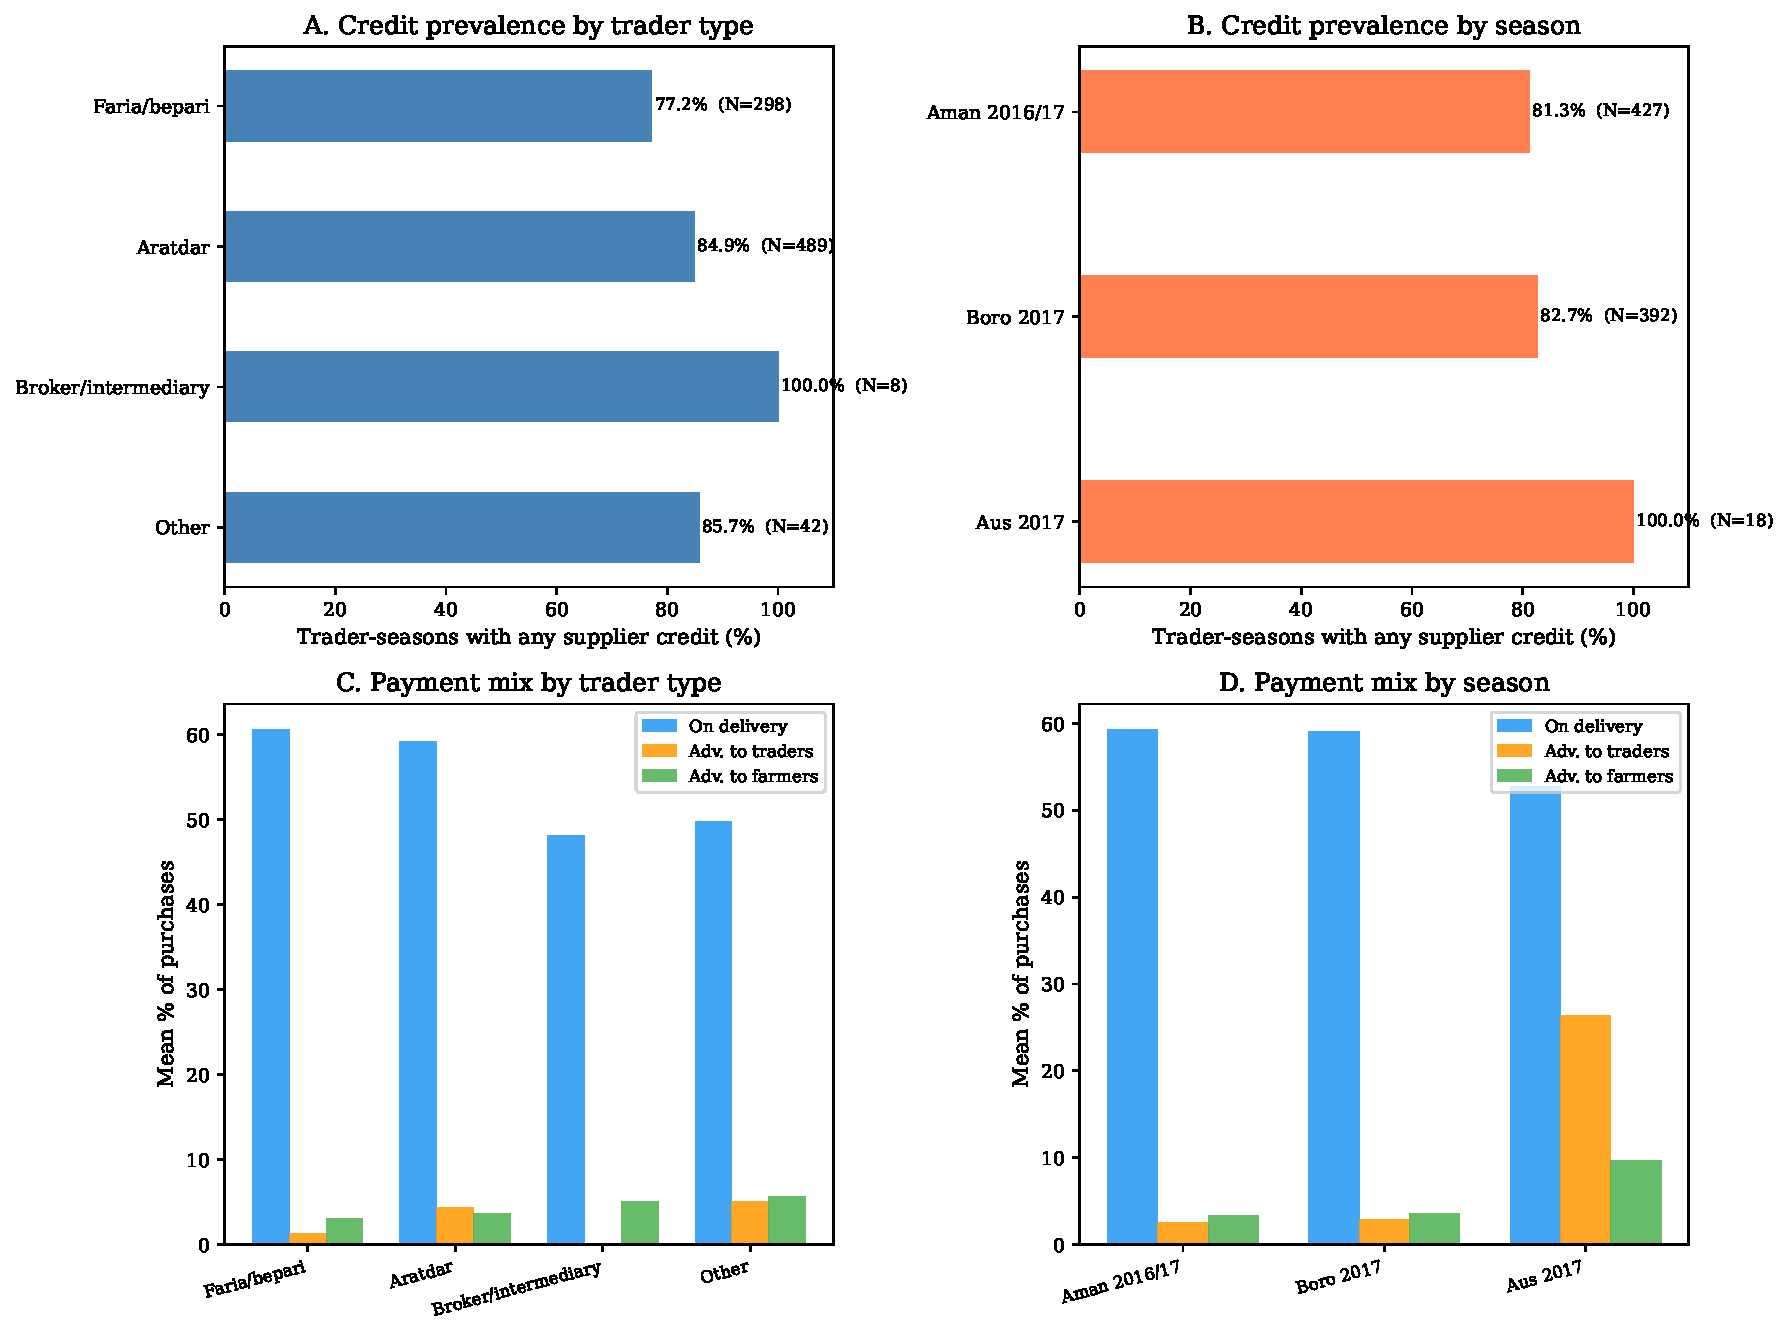
\includegraphics[width=\linewidth]{figures/fig1_credit_prevalence}
  \caption{Credit Prevalence and Payment Mode Composition by Trader Type and Season}
  \label{fig:credit_prev}
  \footnotesize\textit{Notes:} Panels A and B show the percentage of
  trader-season observations with any supplier credit, by trader type and
  season. Panels C and D show mean shares of paddy purchases by payment mode
  (payment on delivery, advance to traders, advance to farmers).
  $N$ as in Table~\ref{tab:credit_by_type}.
\end{figure}

\subsection{Variation by Trader Type}

Credit prevalence and structure vary systematically across trader types
in ways that reflect their structural positions in the paddy supply chain.
Aratdars (commission agents) have the highest credit prevalence (85~percent)
and the longest mean credit duration (18 days), consistent with their hub
role in market networks: as intermediaries facilitating large-volume
transactions, they must sustain simultaneous credit relationships with both
upstream suppliers and downstream buyers across longer inventory cycles.
Faria/bepari, who trade in smaller volumes with faster turnover and less
geographic footprint, show slightly lower prevalence (77~percent) and
shorter duration (12.5 days). Brokers---a small category who facilitate
transactions without taking commodity ownership---show 100~percent credit
use, suggesting that relationship capital, of which credit is a component,
is the primary asset in their business model.
The ``Other'' category stands out for a higher rate of explicit price premia
(22~percent), though the small sample ($N=42$) warrants caution in interpreting
this finding.

\subsection{Seasonal Variation}

Table~\ref{tab:credit_by_season} disaggregates credit by survey season.

\begin{table}[htbp]
  \centering
  \caption{Credit Arrangement Types by Season (Paddy)}
  \label{tab:credit_by_season}
  \begin{singlespace}
  \begin{threeparttable}
    \begin{tabular}{lcccccc}
\toprule
 & \multicolumn{3}{c}{Credit scope (\%)} & \multicolumn{3}{c}{Payment mix (mean \%)} \\
\cmidrule(lr){2-4}\cmidrule(lr){5-7}
Season & None & Some & All & On delivery & Adv.\ to traders & Adv.\ to farmers \\
\midrule
Aman 2016/17 & 18.7 & 71.9 & 9.4 & 59.3 & 2.6 & 3.3 \\
Boro 2017 & 17.3 & 75.3 & 7.4 & 59.1 & 2.9 & 3.5 \\
Aus 2017 & 0.0 & 38.9 & 61.1 & 52.8 & 26.4 & 9.7 \\
\midrule
\textit{All seasons} & 17.7 & 72.8 & 9.6 & 59.1 & 3.3 & 3.6 \\
\addlinespace[2pt]
\multicolumn{7}{p{0.9\textwidth}}{\footnotesize \textit{Note:} Paddy/both trader-seasons only.} \\
\bottomrule
\end{tabular}
    \begin{tablenotes}\footnotesize
      \item \textit{Notes:} Unit of observation is trader $\times$ season.
      Column definitions as in Table~\ref{tab:credit_by_type}.
      Aus 2017 observations are small ($N < 25$); interpret with caution.
    \end{tablenotes}
  \end{threeparttable}
  \end{singlespace}
\end{table}

The two main seasons (Aman and Boro) are strikingly similar: credit
prevalence is 81--83~percent, with 7--9~percent of traders having
all-supplier credit and payment-on-delivery shares of around 59~percent.
The minor Aus season is a dramatic outlier: 61~percent of Aus trader-seasons
report \textit{all}-supplier credit (versus 7--9~percent in main seasons),
and the average advance-to-traders share jumps from 3~percent to 26~percent.
This pattern is consistent with a liquidity-stress mechanism: the Aus harvest
arrives when paddy availability is seasonally low and cash balances are
depleted from the preceding Boro cycle, creating acute working-capital
demand that drives wholesale adoption of credit terms. While the Aus sample
is small ($N \leq 23$), this qualitative shift provides descriptive evidence
that credit intensity responds to seasonal liquidity constraints---a pattern
consistent with credit serving a working-capital function rather than purely
a price-manipulation one.

\subsection{Geographic Variation}

Figure~\ref{fig:credit_map} and Table~\ref{tab:credit_by_district} reveal
substantial geographic segmentation. Near-universal credit prevalence
($\geq$~96~percent) spans geographically diverse districts: Brahmanbaria,
Comilla, and Noakhali in Chittagong division; Naogaon in Rajshahi division;
and Satkhira in Khulna division. In contrast, coastal districts of
Barisal division---Bhola (42~percent), Patuakhali (47~percent), and
Barguna (33~percent)---are below 50~percent.

\begin{figure}[htbp]
  \centering
  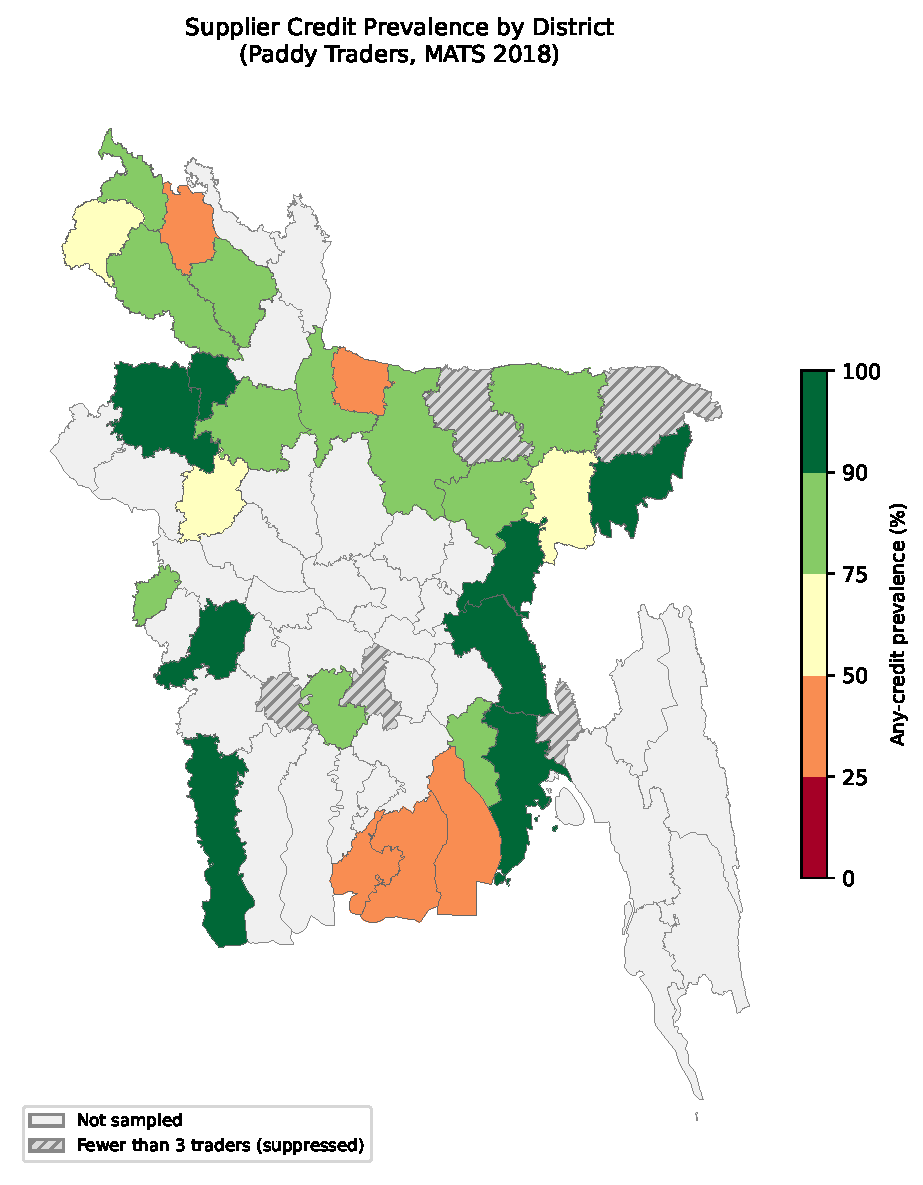
\includegraphics[width=0.8\linewidth]{figures/fig4_credit_map}
  \caption{Supplier Credit Prevalence by District (Paddy Traders, MATS 2018)}
  \label{fig:credit_map}
  \footnotesize\textit{Notes:} Choropleth of the percentage of trader-season
  observations with any supplier credit, by district. Districts shaded grey
  were not sampled in the MATS 2018 paddy trader module; hatched districts
  have fewer than three sampled traders and are suppressed to protect
  respondent confidentiality. Colour scale from
  green (low prevalence) to red (high prevalence).
\end{figure}

\begin{table}[htbp]
  \centering
  \caption{Credit Prevalence by District (Paddy, Selected Districts)}
  \label{tab:credit_by_district}
  \begin{singlespace}
  \begin{threeparttable}
    \begin{tabular}{lcccccc}
\toprule
District & N & Any credit & Credit & On & Adv.\ to & Adv.\ to \\
 & & (\%) & days & delivery & traders & farmers \\
\midrule
\multicolumn{7}{l}{\textit{Highest credit prevalence (top 10 districts)}} \\
\addlinespace[2pt]
Brahmanbaria & 35 & 100.0 & 22.8 & 51.4 & 36.3 & 4.6 \\
Comilla & 9 & 100.0 & 14.1 & 42.2 & 26.7 & 31.1 \\
Joypurhat & 8 & 100.0 & 59.2 & 63.1 & 0.0 & 0.0 \\
Maulvibazar & 34 & 100.0 & 9.5 & 51.0 & 0.6 & 4.4 \\
Noakhali & 23 & 100.0 & 14.0 & 53.0 & 1.7 & 7.6 \\
Naogaon & 29 & 96.6 & 27.6 & 73.8 & 0.0 & 1.9 \\
Satkhira & 52 & 96.2 & 23.8 & 53.0 & 0.0 & 0.5 \\
Jhenaidah & 30 & 93.3 & 15.4 & 40.7 & 0.0 & 8.0 \\
Kishoregonj & 64 & 89.1 & 10.1 & 59.9 & 2.6 & 2.8 \\
Lakshmipur & 9 & 88.9 & 12.5 & 52.5 & 0.6 & 2.5 \\
\addlinespace[4pt]
\multicolumn{7}{l}{\textit{Lowest credit prevalence (bottom 10 districts)}} \\
\addlinespace[2pt]
Bogra & 66 & 77.3 & 22.5 & 64.5 & 0.0 & 0.8 \\
Dinajpur & 8 & 75.0 & 7.3 & 63.3 & 0.0 & 0.0 \\
Thakurgaon & 22 & 72.7 & 9.6 & 24.4 & 10.0 & 4.4 \\
Natore & 18 & 66.7 & 40.0 & 65.8 & 0.0 & 0.0 \\
Habiganj & 12 & 50.0 & 6.2 & 51.7 & 3.3 & 5.0 \\
Patuakhali & 17 & 47.1 & 16.5 & 82.5 & 0.0 & 0.0 \\
Bhola & 19 & 42.1 & 15.2 & 82.5 & 0.0 & 0.0 \\
Barguna & 6 & 33.3 & 30.0 & 72.5 & 0.0 & 0.0 \\
Nilphamari & 12 & 33.3 & 7.2 & 76.2 & 0.0 & 6.2 \\
Sherpur & 14 & 28.6 & 7.0 & 55.0 & 0.0 & 2.5 \\
\addlinespace[2pt]
\multicolumn{7}{p{0.9\textwidth}}{\footnotesize \textit{Note:} Paddy/both trader-seasons only. Credit days and payment shares: means among trader-seasons with any supplier credit. Districts with fewer than 3 sampled traders are omitted.} \\
\bottomrule
\end{tabular}
    \begin{tablenotes}\footnotesize
      \item \textit{Notes:} Top 10 and bottom 10 districts by credit
      prevalence among districts with at least three distinct sampled
      traders (to protect respondent confidentiality).
      Credit duration and advance shares conditional on any credit.
    \end{tablenotes}
  \end{threeparttable}
  \end{singlespace}
\end{table}

The geographic pattern does not map cleanly onto a single agro-ecological
or economic gradient, suggesting that local commercial norms, trading network
structures, and the depth of financial market development---rather than
underlying agricultural conditions alone---shape the prevalence of interlocked
credit. The contrast between the near-universal credit in Chittagong and
Rajshahi division districts and the below-50~percent rates in coastal Barisal
is notable given that both regions are important rice-producing areas. One
possible explanation is that coastal Barisal's more fragmented waterway-based
market structure supports a larger spot market segment where payment on delivery
is feasible, whereas inland market centres with established trading networks
have evolved toward universal credit norms. Credit duration also varies
substantially across districts: traders in Joypurhat average 59 days of
supplier credit, compared with 6--7 days in Dinajpur and Habiganj. This
cross-district variation in the working-capital cycle suggests that credit
duration---like prevalence---reflects local network structure and trading
norms rather than a uniform national market standard.

\subsection{The Local Credit Market Intensity Distribution}

Figure~\ref{fig:credit_dist} shows the distribution of upazila-season
credit shares---the fraction of traders in each local market cell that
use supplier credit.

\begin{figure}[htbp]
  \centering
  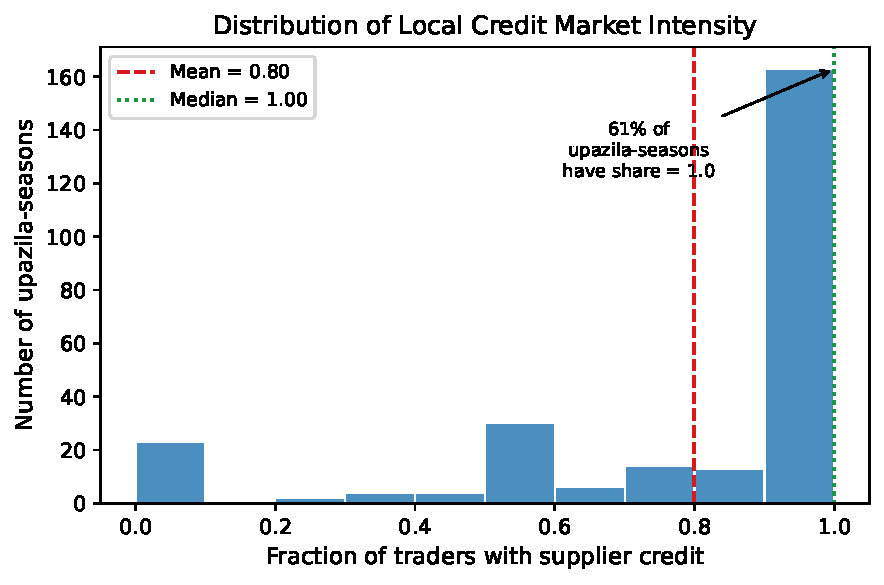
\includegraphics[width=0.75\linewidth]{figures/fig5_credit_dist}
  \caption{Distribution of Local Credit Market Intensity (Upazila-Season Cells)}
  \label{fig:credit_dist}
  \footnotesize\textit{Notes:} Each observation is an upazila $\times$ season
  cell. The x-axis shows the fraction of traders in that cell with any supplier
  credit. The mean is 0.83 and the median is 1.00.
\end{figure}

The distribution is sharply bimodal: the largest single mass (60.8~percent
of upazila-season cells) sits at exactly 1.0---\emph{every} sampled trader
in those local markets uses credit. The remainder spans the full range from
0 to 0.9, with a secondary cluster near 0. This structure has a direct
implication for the Braverman-Stiglitz mechanism: in markets where all
traders use credit, there is no within-market variation in credit status,
and a credit-driven price wedge between credit-using and non-credit-using
traders simply cannot exist by definition. The bimodal distribution suggests
that local credit markets may be characterised by tipping dynamics: once
credit becomes sufficiently prevalent in a market, it is rational for all
remaining buyers to adopt credit terms to remain competitive, driving the
market to a corner solution. Under this interpretation, the 60.8~percent
universal-credit cell share is not evidence of coercive market structure
but of a competitive process that has reached its equilibrium outcome.

The test of price effects is thus driven entirely by the 39.2~percent of
upazila-season cells with mixed credit participation, precisely the cells
where within-market price differentiation by credit status could theoretically
exist. Section~\ref{sec:prices} exploits this variation directly.

%% ─────────────────────────────────────────────────────────────────────────────
\section{Who Uses Credit? Trader Characteristics and Credit Uptake}
\label{sec:determinants}

Table~\ref{tab:determinants} examines the cross-sectional correlates of
credit use at the trader-season level, drawing on trader characteristics
from Modules AB and C1.

\begin{table}[htbp]
  \centering
  \caption{Correlates of Supplier Credit Use (Paddy Traders)}
  \label{tab:determinants}
  \begin{singlespace}
  \begin{threeparttable}
    \begin{tabular}{lcc}
\toprule
& Logit (AME) & LPM \\
& (1) & (2) \\
\midrule
\multicolumn{3}{l}{\textit{Trader characteristics}} \\
\addlinespace[2pt]
Age (years, mean-centred) & 0.001 & 0.000 \\
& (0.001) & (0.002) \\
\addlinespace[2pt]
Schooling (approx.\ years, mean-centred) & -0.011$^{***}$ & -0.011$^{**}$ \\
& (0.004) & (0.005) \\
\addlinespace[2pt]
Years in business (mean-centred) & -0.000 & -0.000 \\
& (0.002) & (0.002) \\
\addlinespace[2pt]
Subsidiary of another business & -0.128$^{***}$ & -0.146$^{***}$ \\
& (0.026) & (0.056) \\
\addlinespace[2pt]
Sole proprietorship & -0.074$^{*}$ & -0.066 \\
& (0.041) & (0.055) \\
\addlinespace[2pt]
Trader type: Aratdar & 0.097$^{***}$ & 0.100$^{**}$ \\
& (0.027) & (0.045) \\
\addlinespace[2pt]
Trader type: Broker/intermediary & {---} & 0.299$^{***}$ \\
&  & (0.070) \\
\addlinespace[2pt]
\midrule
Season FEs & Yes & Yes \\
Observations & 829 & 837 \\
\addlinespace[2pt]
\multicolumn{3}{p{0.72\textwidth}}{\footnotesize \textit{Notes:} Dependent variable: binary indicator for any supplier credit (trader-season). Column (1): logit average marginal effects. Column (2): linear probability model, SE clustered at upazila level. Schooling converts the highest level completed to approximate years. Years in business $= 2018 -$ year the business was established. Reference categories: partnership (ownership), Faria/bepari (trader type). All broker/intermediary trader-seasons report credit, so the broker dummy perfectly predicts the outcome; these observations are dropped from the logit. $^{*}p<0.10$, $^{**}p<0.05$, $^{***}p<0.01$.} \\
\bottomrule
\end{tabular}
    \begin{tablenotes}\footnotesize
      \item \textit{Notes:} Dependent variable: any supplier credit
      (trader-season). Column (1): logit average marginal effects;
      broker/intermediary trader-seasons, all of which report credit, are
      excluded from the logit.
      Column (2): linear probability model with upazila-clustered SEs.
      All specifications include season fixed effects.
      Reference category: Faria/bepari.
      $^{*}p<0.10$, $^{**}p<0.05$, $^{***}p<0.01$.
    \end{tablenotes}
  \end{threeparttable}
  \end{singlespace}
\end{table}

Several patterns emerge. Trader type is the strongest predictor: aratdars
are 10~percentage points more likely to use credit than faria/bepari, and
brokers are 30~percentage points more likely, consistent with their roles
as market intermediaries who anchor credit networks. More educated traders
are \emph{less} likely to use credit: each additional year of schooling is
associated with a reduction of about 1~percentage point. Business tenure,
by contrast, is unrelated to credit use once other characteristics are
held constant. Businesses that are subsidiaries of another enterprise are
13--15~percentage points less likely to report supplier credit. Sole
proprietorships are about 7~percentage points less likely than partnerships
to use credit, but this difference is significant only at the 10~percent
level in the logit and not in the linear probability model.

The pattern on trader type reflects the structural position of different
actors in the paddy supply chain. Aratdars occupy hub positions from which
credit flows both upstream (to faria) and downstream (from wholesalers),
making credit integral to their intermediation function. Brokers, whose
business model depends entirely on maintaining active relationships on both
sides of each transaction, show the highest prevalence---relationship
capital, of which credit is a component, is their primary asset. This
pattern closely mirrors findings from Pakistan's grain markets, where
\textit{arthis} (commission agents) serve simultaneously as financiers and
exclusive output buyers \citep{haq_etal2013}, and from Punjab, India,
where interlinked credit through arhatiyas is concentrated at the
commission-agent level of the market hierarchy \citep{gill2004}.

The negative association between education and credit use is consistent
with two mechanisms. First, more educated traders may have greater access
to formal financial products---bank credit, microfinance---that substitute
for relationship-based trade credit \citep{conning_udry2007}. Second,
traders with higher education may have accumulated stronger market
reputations and broader trading networks that reduce their dependence on
any single buyer's credit. That business tenure itself shows no association
with credit use suggests that what matters is traders' human and financial
capital rather than experience in the trade as such.

The lower credit use among subsidiary businesses is particularly notable.
A trading business that belongs to a larger enterprise can draw on the
parent firm's working capital and banking relationships, and therefore has
less need for credit from its suppliers. The coefficient is consistent with
traders substituting away from relationship-based trade credit when
alternative finance is available, in line with evidence from microfinance
studies showing that access to formal credit partially displaces informal
credit in agricultural markets \citep{karlan_etal2014}.

Taken together, these patterns characterise supplier credit as an institution
embedded in informal, relationship-based trading networks, disproportionately
relied upon by traders with fewer alternative sources of finance and greater
dependence on bilateral buyer relationships for market access.

%% ─────────────────────────────────────────────────────────────────────────────
\section{Does Credit Depress Procurement Prices?}
\label{sec:prices}

\subsection{Estimation Strategy}

Let $p_{its}$ denote the log of the average monthly paddy procurement price
(BDT/kg) for trader $i$ in month $t$ of season $s$. The estimating equation is:

\begin{equation}
  \label{eq:ols}
  p_{its} = \alpha + \boldsymbol{\beta}' \mathbf{C}_{is}
            + \mu_u + \lambda_s + \delta_t + \varepsilon_{its},
\end{equation}

where $\mathbf{C}_{is}$ is a vector of credit arrangement indicators at the
trader-season level, and $\mu_u$, $\lambda_s$, $\delta_t$ absorb upazila,
season, and month fixed effects, respectively. Standard errors are clustered
at the upazila level. The identifying assumption is that, within the same
upazila-season, credit status is uncorrelated with the error term conditional
on fixed effects.

To address potential endogeneity---stronger, more established traders may
simultaneously receive more credit and pay higher prices through quality
selection---we instrument individual credit receipt with the leave-one-out
average credit rate among other traders in the same upazila-season:

\begin{equation}
  \label{eq:instrument}
  Z_{is} = \frac{\sum_{j \neq i,\; u(j)=u(i),\; s(j)=s} C_{js}}{N_{us}-1}.
\end{equation}

This instrument captures the local credit culture or market norm while
excluding the own trader's decision. Because the instrument varies at the
upazila-season level, we replace upazila fixed effects with district fixed
effects in the IV specification. The exclusion restriction requires that
the local credit norm affects procurement prices only through individual
credit receipt, which is plausible if local norms proxy for network
embeddedness rather than directly for price levels.

\subsection{OLS Results}

Table~\ref{tab:ols} presents OLS estimates.

\begin{table}[htbp]
  \centering
  \caption{OLS Estimates: Effect of Supplier Credit on Log Paddy Procurement Price}
  \label{tab:ols}
  \begin{singlespace}
  \begin{threeparttable}
    \begin{tabular}{lcccc}
\toprule
& (1) & (2) & (3) & (4) \\
\midrule
Any supplier credit & -0.0134 &  & -0.0087 & -0.0128 \\
& (0.0169) &  & (0.0164) & (0.0155) \\
\addlinespace[2pt]
\quad Some suppliers &  & -0.0126 &  &  \\
&  & (0.0167) &  &  \\
\addlinespace[2pt]
\quad All suppliers &  & -0.0313 &  &  \\
&  & (0.0321) &  &  \\
\addlinespace[2pt]
\quad Adv.\ to farmers (\% purch.) &  &  & -0.0016 &  \\
&  &  & (0.0014) &  \\
\addlinespace[2pt]
\quad Adv.\ to traders (\% purch.) &  &  & -0.0009 &  \\
&  &  & (0.0009) &  \\
\addlinespace[2pt]
\midrule
Observations & 4,354 & 4,354 & 4,354 & 4,354 \\
$R^2$ & 0.422 & 0.422 & 0.424 & 0.456 \\
Upazila FEs & Yes & Yes & Yes & Yes \\
Season \& month FEs & Yes & Yes & Yes & Yes \\
Variety FEs & No & No & No & Yes \\
\addlinespace[2pt]
\multicolumn{5}{p{0.85\textwidth}}{\footnotesize \textit{Notes:} Dependent variable: log paddy procurement price (BDT/kg). Standard errors (in parentheses) clustered at the upazila level. Sample restricted to paddy/both trader-season-months with price between 5 and 50 BDT/kg. $^{*}p<0.10$, $^{**}p<0.05$, $^{***}p<0.01$.} \\
\bottomrule
\end{tabular}
    \begin{tablenotes}\footnotesize
      \item \textit{Notes:} Dependent variable: log(monthly average paddy
      procurement price, BDT/kg). All specifications include upazila, season,
      and month fixed effects. Column (4) additionally includes paddy variety
      fixed effects. Standard errors clustered at the upazila level in
      parentheses. *** $p<0.01$, ** $p<0.05$, * $p<0.1$.
    \end{tablenotes}
  \end{threeparttable}
  \end{singlespace}
\end{table}

The upazila fixed effects absorb all time-invariant characteristics of local
paddy markets, including market infrastructure, trader composition, and
the general level of buyer competition. Month fixed effects absorb
aggregate seasonal price variation---the post-harvest price drop and
pre-harvest scarcity premium that are characteristic of Bangladesh rice
markets. The identifying variation is therefore the within-upazila,
within-month, cross-trader difference in credit status: the closest
available approximation to comparing otherwise similar traders in the
same local market at the same time.

Across all four specifications, credit arrangement indicators are small and
statistically indistinguishable from zero. The any-credit binary in Column (1)
yields $-0.013$ (SE $= 0.017$, $p = 0.43$), implying a 1.3~percent lower
price in seasons with supplier credit---not distinguishable from zero.
Scope dummies (Column 2), payment-share variables (Column 3), and variety
controls (Column 4) all leave the inference unchanged. The $R^2$ of
0.42--0.46 indicates that location, season, and variety account for
nearly half of the variation in monthly procurement prices; credit
arrangement variables contribute essentially nothing beyond these controls.

The null result is precisely estimated enough to rule out economically
large price effects. The 95~percent confidence interval in Column (1)
excludes price discounts larger than about 4.5~percent ($-0.047$ log
points). By comparison, the Braverman-Stiglitz mechanism would predict
that an implicit interest rate on trade credit should translate into a
procurement price discount of similar magnitude. Given informal credit
rates in Bangladesh agriculture of roughly 30--60~percent per annum and
typical credit durations of 10--18 days observed in the MATS, the
implied price discount per transaction would be approximately
1--3~percent---within the confidence interval but not ruled out at point
estimates near zero. The results therefore do not conclusively falsify
the mechanism but are inconsistent with it operating at scale within
local markets.

\subsection{IV Results and Heterogeneity}

Table~\ref{tab:iv} reports the IV robustness check.

\begin{table}[htbp]
  \centering
  \caption{IV Robustness: 2SLS with Leave-One-Out Upazila-Season Credit Rate}
  \label{tab:iv}
  \begin{singlespace}
  \begin{threeparttable}
    \begin{tabular}{lccc}
\toprule
& \multicolumn{2}{c}{OLS} & 2SLS \\
\cmidrule(lr){2-3}
& Upazila FE & District FE & District FE \\
& (1) & (2) & (3) \\
\midrule
Any supplier credit & -0.0134 & -0.0198 & -0.0422 \\
& (0.0169) & (0.0180) & (0.0371) \\
\addlinespace[4pt]
\midrule
Observations & 4,354 & 4,351 & 4,351 \\
Upazila FEs & Yes & No & No \\
District FEs & No & Yes & Yes \\
Season \& month FEs & Yes & Yes & Yes \\
First-stage $F$ & & & 1365.2 \\
\addlinespace[2pt]
\multicolumn{4}{p{0.75\textwidth}}{\footnotesize \textit{Notes:} Dependent variable: log paddy procurement price. Instrument (col.\ 3): leave-one-out upazila-season credit share. SE clustered at upazila level. $^{*}p<0.10$, $^{**}p<0.05$, $^{***}p<0.01$.} \\
\bottomrule
\end{tabular}
    \begin{tablenotes}\footnotesize
      \item \textit{Notes:} Dependent variable: log(monthly average paddy
      procurement price, BDT/kg). All specifications include district, season,
      and month fixed effects. Standard errors clustered at the upazila level.
      *** $p<0.01$, ** $p<0.05$, * $p<0.1$.
    \end{tablenotes}
  \end{threeparttable}
  \end{singlespace}
\end{table}

The instrument's exceptional strength ($F = 1{,}365$) reflects the high spatial
correlation of credit norms within upazila-season cells: if most traders in
a local market use credit, the remainder are very likely to as well. This
homogeneity is a direct consequence of the bimodal credit distribution documented
in Section~\ref{sec:descriptive}---in the modal market cell, all traders use
credit, making the LOO rate a near-perfect predictor of own credit receipt.

The 2SLS estimate of $-0.042$ (SE $= 0.037$, $p = 0.26$) is approximately
three times larger in magnitude than the OLS estimate, consistent with
positive OLS attenuation bias: better-connected, more established traders
receive more credit and simultaneously pay higher prices through quality
selection and network access. Correcting for this upward bias does not bring
the IV estimate to significance. The exclusion restriction requires that
local credit norms affect prices only through individual credit receipt,
not through other channels. This restriction would be violated if high-credit
upazilas have structurally different market competition or pricing norms;
we cannot directly test this, but the consistent null across specifications
with varying fixed effects structures provides some reassurance.

Table~\ref{tab:heterogeneity} confirms the null across subgroups. Panel A
stratifies by market credit intensity, comparing upazila-seasons above and
below the median credit share. Neither group shows a significant effect.
Panel B focuses on the mixed-market subsample---upazila-seasons where some
but not all traders use credit---precisely the cells where within-market
price differentiation by credit status could theoretically exist. Even here
the effect is not distinguishable from zero, indicating that the null is not
solely attributable to the universal-credit majority of market cells.

\begin{table}[htbp]
  \centering
  \caption{Heterogeneous Price Effects of Supplier Credit}
  \label{tab:heterogeneity}
  \begin{singlespace}
  \begin{threeparttable}
    \begin{tabular}{lc}
\toprule
& Log price \\
\midrule
\multicolumn{2}{l}{\textit{Panel A: Interaction with local credit market intensity (district FEs)}} \\
\addlinespace[2pt]
Any supplier credit (at mean local share) & -0.0276 \\
& (0.0207) \\
Local credit share (mean-centred) & 0.0255 \\
& (0.0502) \\
\quad Credit $\times$ local share & -0.0854 \\
& (0.0647) \\
\addlinespace[2pt]
Observations & 4,354 \\
$R^2$ & 0.279 \\
\addlinespace[6pt]
\multicolumn{2}{l}{\textit{Panel B: Mixed-market subsample (local credit share $<$ 100\%, district FEs)}} \\
\addlinespace[2pt]
Any supplier credit (mixed-market upazila-seasons) & -0.0191 \\
& (0.0174) \\
\addlinespace[2pt]
Observations & 1,970 \\
\addlinespace[6pt]
\multicolumn{2}{l}{\textit{Panel C: Heterogeneity by trader type (upazila FEs; ref.\ = Faria/bepari)}} \\
\addlinespace[2pt]
Any credit & -0.0048 \\
& (0.0271) \\
\quad $\times$ Aratdar & -0.0246 \\
& (0.0367) \\
\quad $\times$ Broker/intermediary & 0.0225 \\
& (0.0339) \\
\addlinespace[2pt]
Observations & 4,354 \\
\addlinespace[2pt]
\multicolumn{2}{p{0.7\textwidth}}{\footnotesize \textit{Notes:} Panels A and B use district FEs; Panel C uses upazila FEs. Standard errors clustered at upazila level. $^{*}p<0.10$, $^{**}p<0.05$, $^{***}p<0.01$.} \\
\bottomrule
\end{tabular}
    \begin{tablenotes}\footnotesize
      \item \textit{Notes:} Panels A and B use district, season, and month
      fixed effects; Panel C uses upazila, season, and month fixed effects.
      Standard errors clustered at upazila level.
      $^{*}p<0.10$, $^{**}p<0.05$, $^{***}p<0.01$.
    \end{tablenotes}
  \end{threeparttable}
  \end{singlespace}
\end{table}

\subsection{Credit and Price Variance}

If credit does not compress price \emph{levels}, it might still reduce
within-season price \emph{volatility} by smoothing working-capital
constraints. Table~\ref{tab:price_variance} tests this. The evidence points
in the opposite direction: traders who use credit face \emph{higher} price
standard deviation ($+$0.25 BDT/kg, $p = 0.08$) and coefficient of
variation ($+$1.18 percentage points, $p = 0.05$). Column (3) shows this
pattern is driven by ``some-credit'' traders, who transact under mixed terms
across purchases.

\begin{table}[htbp]
  \centering
  \caption{Supplier Credit and Within-Season Price Variance}
  \label{tab:price_variance}
  \begin{singlespace}
  \begin{threeparttable}
    \begin{tabular}{lccc}
\toprule
& Price SD & Price CV & Price CV \\
& (BDT/kg) & (\%) & (\%) \\
& (1) & (2) & (3) \\
\midrule
Any supplier credit & 0.2538$^{*}$ & 1.1781$^{*}$ &  \\
& (0.1432) & (0.6067) &  \\
\addlinespace[2pt]
\quad Some suppliers &  &  & 1.2085$^{**}$ \\
&  &  & (0.5979) \\
\addlinespace[2pt]
\quad All suppliers &  &  & 0.5887 \\
&  &  & (1.3487) \\
\addlinespace[2pt]
\midrule
Observations & 822 & 822 & 822 \\
$R^2$ & 0.597 & 0.604 & 0.604 \\
Upazila FEs & Yes & Yes & Yes \\
Season FEs  & Yes & Yes & Yes \\
\addlinespace[2pt]
\multicolumn{4}{p{0.75\textwidth}}{\footnotesize \textit{Notes:} Unit of observation is trader $\times$ season, restricted to trader-seasons with $\geq 2$ active procurement months ($N=822$). Price CV $=$ (SD/mean) $\times$ 100. SE clustered at upazila level. $^{*}p<0.10$, $^{**}p<0.05$, $^{***}p<0.01$.} \\
\bottomrule
\end{tabular}
    \begin{tablenotes}\footnotesize
      \item \textit{Notes:} Unit of observation is trader $\times$ season
      with $\geq 2$ active procurement months ($N = 822$).
      Price CV $=$ (SD/mean) $\times$ 100. Upazila and season fixed effects.
      Standard errors clustered at upazila level.
      $^{*}p<0.10$, $^{**}p<0.05$, $^{***}p<0.01$.
    \end{tablenotes}
  \end{threeparttable}
  \end{singlespace}
\end{table}

Rather than indicating a disciplinary role for credit in price formation,
the positive variance relationship suggests that credit-enabled procurement
spans a broader range of market conditions. Traders with credit access
can purchase across more time periods---at harvest when prices are low
and during scarcity when prices are high---increasing their exposure to
price swings. A cash-constrained trader, by contrast, may be limited to
purchasing in narrow windows when working capital is available and prices
are predictable. Column (3) provides suggestive evidence for this
mechanism: the variance premium is largest for ``some-credit'' traders,
who purchase under mixed terms across different counterparties, consistent
with a broadened procurement window rather than a stabilising credit effect.

This finding connects to \citet{barrett2008}'s argument that liquidity
constraints at harvest force distress selling at depressed prices, while
\citet{stephens_barrett2011} show that credit-using traders in Kenya access
a broader market range. Both are consistent with the picture emerging
here: credit functions as a market-access enabler, expanding the price
distribution a trader is exposed to, rather than as a stabilising or
suppressive force on the prices they receive. The policy implication is
that the welfare calculus of credit access is more nuanced than either the
Braverman-Stiglitz suppression narrative or the simple liquidity-smoothing
narrative suggests.

%% ─────────────────────────────────────────────────────────────────────────────
\section{Market Structure Implications and Policy Relevance}
\label{sec:implications}

\subsection{Why No Price Effect? Three Interpretations}

The null price result is interpretable through three non-exclusive mechanisms,
each with distinct policy implications.

\textit{Competitive credit markets.} With 82~percent credit prevalence and
a 60.8~percent share of upazila-season cells at full participation, supplier
credit is a standard feature of market entry rather than a monopolistic
privilege. Where all traders in a market use credit, credit cannot generate
within-market price differentiation regardless of the power structure between
buyers and sellers. The near-universal prevalence may itself reflect a
competitive equilibrium in which credit terms have been standardised across
buyers: as \citet{basu1983} shows theoretically, interlinkage can arise
as a competitive equilibrium even without a dominant lender, because it
solves shared enforcement and information problems. In Bangladesh's densely
traded rice markets, where multiple buyer types (faria, aratdars, wholesalers)
compete for paddy in most market centres, this competitive equilibration
is plausible. \citet{rahman_etal2020} find significant but far from monopolistic
markups among Bangladesh millers and wholesalers, consistent with imperfect
but not monopsonistic competition at the end of the supply chain.
The credit norm may therefore be evidence of convergence to a common
market institution rather than of exploitation.

\textit{Relationship capital.} Interlocked credit may function primarily as
a relational contract offering supply certainty, quality enforcement,
and priority access when supply is tight
\citep{casaburi_macchiavello2019, blouin_macchiavello2019,
macchiavello_morjaria2015}. Under this interpretation, the value of
the credit relationship to the buyer is embodied in reduced search costs
and guaranteed supply rather than in a below-market procurement price.
The buyer's willingness to extend credit signals relationship depth and
creates incentives for the seller to maintain delivery commitments and
quality standards. This interpretation is supported by our finding that
94.5~percent of credit-holding traders report no explicit price premium---the
credit is embedded in the relationship without separate pricing, consistent
with credit being valued by both parties as a relational device rather
than extracted as an implicit interest payment. The relational contracting
interpretation also helps explain the persistence of credit alongside
mobile money: if credit's primary function is relationship signalling
and supply commitment rather than liquidity provision, digital payment
instruments that address only the liquidity dimension would not substitute
for it.

\textit{Measurement.} The outcome variable is the trader's average monthly
procurement price across all sources and varieties. If a trader procures
some paddy on credit at a small discount and other paddy at market price,
the average masks the transaction-level effect. Transaction-level panel
data tracking individual buyer-seller pairs would be needed to detect
such effects.

\subsection{The Dual Market and Its Welfare Implications}

The finding that 94.5~percent of credit-holding traders report no explicit
price premium, while the remaining 5.5~percent face implied annual rates of
51~percent, is consistent with a dual credit market \citep{hoff_stiglitz1990}.
In the dominant implicit segment, credit is embedded in trade relationships
and priced through relationship rents---supply loyalty, first-call rights,
enforcement of delivery commitments---that are not separately visible in
procurement price data. In the residual explicit segment, credit carries a
high stated price, potentially reflecting transactions outside established
networks or between parties without the relationship depth to sustain
fully implicit pricing.

The welfare implications differ sharply between segments. The implicit
segment is most consistent with a relational equilibrium that may be
Pareto-improving relative to spot market trading: both buyer and seller
benefit from the supply certainty and delivery enforcement the relationship
provides. This is analogous to findings from other relationship markets
where long-term contracts involve implicit subsidies that are sustained by
the value both parties derive from relationship continuity
\citep{macchiavello_morjaria2015}. The explicit segment, where rates of
51~percent per annum are documented, is more likely to reflect genuine
credit constraint---a seller with few alternatives paying above-market rates
for essential working capital. The implied annual rate is substantially
above formal lending rates but is consistent with evidence from across
South Asia on informal moneylender rates, which typically range from 36
to 120~percent per annum \citep{hoff_stiglitz1990}.

The policy-relevant question is the size of each segment. At 5.5~percent
of trader-seasons, the high-rate explicit segment is a small minority in
aggregate terms, but concentrated among specific trader types and regions.
Given that the MATS captures only formally present market-centre traders,
the more financially vulnerable faria operating at village level---who
are less well represented in the sample---may face a higher share of
explicit-price credit, implying that aggregate 5.5~percent is a lower
bound on the prevalence of the welfare-concerning segment.

\subsection{Lock-in Without Price Wedges}

The most important policy-relevant finding is that credit's competitive effects
can operate without observable price wedges. Lock-in to a buyer's credit
network limits the effective choice set of upstream sellers, reducing
the number of competitive buyers even when many are physically present.
\citet{crow_murshid1994} describe this mechanism explicitly for Bangladesh's
grain markets as ``economic returns to social power'': merchants' finance
creates vertical ties that constrain supplier mobility without generating
price differentials visible in cross-sectional data.
\citet{murshid2015} revisits these markets two decades later and finds
that while traditional interlinking has partially transformed, new forms
of dependence (contract milling, input supply tied to output procurement)
have replaced older credit-commodity links, suggesting that the lock-in
mechanism is persistent even as its specific institutional form evolves.

The determinants analysis reinforces this interpretation. Traders with
less schooling and those whose businesses are not part of a larger
enterprise are more likely to rely on supplier credit, suggesting that
credit relationships are more deeply embedded among those with limited
alternative sources of finance. These are precisely the traders for whom
exit from a credit relationship would be most costly and for whom lock-in
effects would be strongest, even in the absence of observable price
differences.

Experimental evidence from other markets supports this mechanism.
\citet{bergquist_dinerstein2020} find that grain traders in Kenya sustain
significant markups even when multiple competitors are present, consistent
with tacit collusion enabled by relational structures. While their work
is not directly about interlocked credit, it illustrates how relationship-based
market structures can sustain rents above the competitive level without
generating observable price variation in standard cross-sectional data.

\subsection{Policy Implications}

Several policy implications follow from these findings.

\textit{Credit transparency and disclosure.} The 5.5~percent of traders
in the explicit pricing segment---likely the most welfare-relevant group---face
opaque credit terms embedded in commodity transactions. Price transparency
requirements and disclosure rules for trade credit, modelled on consumer
credit regulation, could improve welfare in this segment without disrupting
the larger implicit credit market that appears to serve legitimate working
capital functions.

\textit{Alternative finance access.} The lower credit use among subsidiary
businesses and more educated traders suggests that access to alternative
finance reduces reliance on relationship-based trade credit. Policies that
improve MSME access to bank and MFI credit could reduce traders' dependence
on potentially extractive credit relationships, particularly for smaller
faria/bepari traders.

\textit{Targeting of interventions.} The strong seasonal and geographic
heterogeneity in credit prevalence---from 100~percent in northeastern
districts to below 35~percent in coastal Barisal, and from 7~percent
all-supplier credit in main seasons to 61~percent in the Aus season---argues
against one-size-fits-all credit market interventions. Seasonal liquidity
support targeted at the Aus period and geographic targeting toward coastal
low-credit districts may be more effective than national-level credit
expansion.

\textit{Limits of price-based monitoring.} Given that credit effects operate
primarily through relationship lock-in and supply certainty rather than
observable price wedges, price-based competition monitoring of agricultural
procurement markets will systematically miss the welfare effects of credit
interlocking. Effective market oversight requires data on relationship
structures and market access, not just prices.

%% ─────────────────────────────────────────────────────────────────────────────
\section{Conclusion}
\label{sec:conclusion}

This paper provides the first large-scale, nationally distributed
characterisation of interlocked credit in Bangladesh's rice trading sector. Using a purpose-designed
trader survey that directly measures credit arrangement types, payment mode
composition, trader characteristics, and monthly procurement prices, we document
that supplier credit is near-universal (82~percent of paddy trader-seasons),
primarily implicit in its pricing (94.5~percent report no explicit price premium),
and most common among traders with less schooling, without a parent business,
and occupying central positions in trading networks.

Despite the pervasiveness of credit interlocking, we find no evidence that
it depresses procurement prices within local markets. OLS and IV estimates
are uniformly small and insignificant. A key structural reason is that the
majority of local market cells have full credit participation, precluding
within-market price differentiation by credit status. Credit appears to
function primarily as relationship capital, consistent with relational
contracting rather than surplus extraction through price manipulation.

Two findings stand out as particularly policy-relevant. First, the thin
segment of traders facing explicit price premia---at implied rates of 51~percent
per annum---represents a potential welfare concern that current price-focused
market monitoring would miss. Second, the positive association between credit
use and price variance suggests that credit enables broader market participation
rather than stabilising procurement conditions, qualifying the conventional
welfare narrative of credit smoothing in agricultural supply chains.

Several limitations of the current analysis merit acknowledgment. The MATS
is a cross-sectional survey, preventing analysis of within-trader changes
in credit use over time. The price variable measures traders' average
monthly procurement price across all sources, potentially masking
transaction-level effects that would only be visible in matched buyer-seller
panel data. The LOO instrument, while statistically powerful, rests on an
exclusion restriction that cannot be directly tested---local credit norms
could affect prices through channels other than individual credit receipt.
The trader sample's snowball construction---drawn from millers' reported key
buyers and suppliers---over-represents traders who deal directly with millers
and under-represents terminal traders selling to consumers, which may bias
estimates of credit prevalence toward the miller-linked segment of the
trading network \citep{dorosh_etal2021}.

These limitations suggest a clear research agenda. The most important
missing piece is transaction-level panel data linking individual buyer-seller
pairs over time, as in \citet{casaburi_macchiavello2019}'s dairy market
study---data that would allow identification of whether credit terms predict
future price outcomes within bilateral relationships. Second, quasi-experimental
variation from mobile money rollouts, MFI program expansions, or agricultural
credit schemes would enable causal analysis of formal credit access on
trade credit reliance, testing directly whether financial inclusion substitutes
for interlocked credit. Third, extending the analysis to rice traders and
downstream value chain stages would clarify whether credit lock-in at
the paddy procurement level propagates to consumer prices or is absorbed
in millers' margins.

These results reinforce the case for high-frequency, transaction-level
data collection in agricultural market monitoring systems: the mechanisms
through which credit affects market performance are subtler than observable
price differences, operating through supply security, effective competition,
and relationship rents. Standard price-monitoring programs will systematically
fail to detect the welfare costs of credit interlocking. Richer
administrative and survey data---and the quasi-experimental variation it
enables---are needed for more definitive welfare analysis of interlocked
credit in South Asian grain markets and across agricultural value chains
in developing economies more broadly.

%% ─────────────────────────────────────────────────────────────────────────────
\section*{Declaration of competing interests}

The author declares no known competing financial interests or personal
relationships that could have appeared to influence the work reported in
this paper.

%% ─────────────────────────────────────────────────────────────────────────────
\bibliographystyle{elsarticle-harv}
\bibliography{references}

%% ─────────────────────────────────────────────────────────────────────────────
\appendix

\section{Full Upazila-Level Credit Prevalence}
\label{app:upazila}

Table~\ref{tab:upazila} reports credit prevalence, mean credit duration,
and mean payment-share variables for all upazilas with at least three
distinct traders in the paddy subsample, sorted by credit prevalence; $N$ is
the number of trader-season observations. Upazilas with fewer than three
sampled traders are omitted to protect respondent confidentiality.

\begin{longtable}{lrrrrrr}
\caption{Upazila-Level Credit Prevalence (Paddy)} \label{tab:upazila} \\
\toprule
Upazila & $N$ & Any credit & Credit & On & Adv.\ to & Adv.\ to \\
& & (\%) & days & delivery & traders & farmers \\
\midrule
\endfirsthead
\multicolumn{7}{l}{\tablename\ \thetable{} -- continued} \\
\toprule
Upazila & $N$ & Any credit & Credit & On & Adv.\ to & Adv.\ to \\
& & (\%) & days & delivery & traders & farmers \\
\midrule
\endhead
\midrule \multicolumn{7}{r}{\footnotesize Continued on next page} \\
\endfoot
\bottomrule
\endlastfoot
Ashuganj & 24 & 100.0 & 24.2 & 54.2 & 36.7 & 0.0 \\
Boda & 8 & 100.0 & 10.5 & 58.8 & 0.0 & 5.0 \\
Derai & 8 & 100.0 & 6.8 & 53.1 & 10.6 & 3.5 \\
Fulbaria & 6 & 100.0 & 8.8 & 79.2 & 0.0 & 0.0 \\
Haluaghat & 12 & 100.0 & 25.7 & 58.3 & 0.0 & 0.0 \\
Hossainpur & 6 & 100.0 & 7.7 & 47.5 & 0.0 & 0.0 \\
Ishwarganj & 6 & 100.0 & 9.5 & 46.7 & 0.0 & 0.0 \\
Jhenaidah Sadar & 10 & 100.0 & 21.4 & 39.0 & 0.0 & 0.0 \\
Kalaroa & 14 & 100.0 & 22.1 & 46.2 & 0.0 & 0.3 \\
Kaliganj & 16 & 100.0 & 11.8 & 36.9 & 0.0 & 14.0 \\
Kamalganj & 10 & 100.0 & 7.8 & 58.0 & 2.0 & 2.0 \\
Kaunia & 6 & 100.0 & 7.3 & 57.8 & 11.7 & 10.0 \\
Kishoreganj Sadar & 18 & 100.0 & 12.2 & 61.7 & 1.7 & 1.2 \\
Kulaura & 4 & 100.0 & 14.8 & 50.0 & 0.0 & 5.0 \\
Mahadebpur & 8 & 100.0 & 38.2 & 65.6 & 0.0 & 0.0 \\
Maulvibazar Sadar & 9 & 100.0 & 5.3 & 63.3 & 0.0 & 6.7 \\
Mujib Nagar & 6 & 100.0 & 11.2 & 51.7 & 0.0 & 15.0 \\
Phulpur & 12 & 100.0 & 13.8 & 75.4 & 2.1 & 5.0 \\
Rangpur Sadar & 6 & 100.0 & 8.0 & 66.7 & 0.0 & 0.0 \\
Sapahar & 5 & 100.0 & 9.8 & 78.0 & 0.0 & 8.0 \\
Satkhira Sadar & 32 & 100.0 & 23.9 & 56.2 & 0.0 & 0.0 \\
Shibganj & 8 & 100.0 & 10.6 & 53.8 & 0.0 & 0.0 \\
Singra & 6 & 100.0 & 35.0 & 55.8 & 0.0 & 0.0 \\
Sreemangal & 9 & 100.0 & 13.9 & 37.2 & 0.0 & 5.6 \\
Subarnachar & 18 & 100.0 & 11.4 & 55.6 & 2.2 & 6.9 \\
Tarakanda & 8 & 100.0 & 14.8 & 65.6 & 0.0 & 0.0 \\
Karimganj & 14 & 92.9 & 11.0 & 66.5 & 0.0 & 0.8 \\
Gangni & 25 & 92.0 & 11.7 & 53.9 & 0.7 & 15.2 \\
Patnitala & 10 & 90.0 & 23.9 & 74.4 & 0.0 & 1.6 \\
Jamalpur Sadar & 34 & 88.2 & 11.7 & 71.5 & 0.0 & 1.5 \\
Gopalganj Sadar & 8 & 87.5 & 10.4 & 74.3 & 2.9 & 0.0 \\
Sherpur & 8 & 87.5 & 19.6 & 62.3 & 0.0 & 0.0 \\
Muktagachha & 14 & 85.7 & 13.7 & 69.2 & 0.0 & 0.0 \\
Pirganj & 26 & 84.6 & 7.3 & 54.8 & 9.1 & 5.5 \\
Nandail & 12 & 83.3 & 9.0 & 50.0 & 0.0 & 0.0 \\
Sunamganj Sadar & 6 & 83.3 & 9.0 & 59.0 & 2.0 & 4.0 \\
Bishwambarpur & 11 & 81.8 & 7.9 & 62.2 & 0.0 & 3.6 \\
Nandigram & 22 & 81.8 & 22.4 & 71.7 & 0.0 & 0.0 \\
Adamdighi & 8 & 75.0 & 39.2 & 61.7 & 0.0 & 0.0 \\
Jamalganj & 8 & 75.0 & 8.5 & 53.3 & 0.0 & 10.8 \\
Pakundia & 8 & 75.0 & 3.7 & 60.8 & 10.0 & 8.3 \\
Meherpur Sadar & 14 & 71.4 & 19.4 & 57.5 & 2.0 & 7.5 \\
Mitha Pukur & 14 & 71.4 & 11.6 & 61.0 & 0.0 & 0.0 \\
Galachipa & 3 & 66.7 & 20.0 & 85.0 & 0.0 & 0.0 \\
Pirgachha & 17 & 64.7 & 8.0 & 54.5 & 0.0 & 1.8 \\
Kalapara & 5 & 60.0 & 12.3 & 80.0 & 0.0 & 0.0 \\
Lalmohan & 7 & 57.1 & 17.5 & 82.5 & 0.0 & 0.0 \\
Melandaha & 18 & 55.6 & 10.3 & 52.0 & 1.0 & 3.0 \\
Baliadangi & 8 & 50.0 & 12.5 & 65.0 & 0.0 & 0.0 \\
Dashmina & 4 & 50.0 & 17.5 & 85.0 & 0.0 & 0.0 \\
Gabtali & 8 & 50.0 & 11.0 & 62.5 & 0.0 & 7.5 \\
Habiganj Sadar & 8 & 50.0 & 7.0 & 47.5 & 0.0 & 2.5 \\
Baraigram & 10 & 40.0 & 45.0 & 75.0 & 0.0 & 0.0 \\
Mymensingh Sadar & 10 & 40.0 & 11.0 & 72.5 & 0.0 & 0.0 \\
Amtali & 6 & 33.3 & 30.0 & 72.5 & 0.0 & 0.0 \\
Bhola Sadar & 6 & 33.3 & 10.0 & 80.0 & 0.0 & 0.0 \\
Char Fasson & 6 & 33.3 & 16.0 & 85.0 & 0.0 & 0.0 \\
Domar & 6 & 33.3 & 6.5 & 82.5 & 0.0 & 0.0 \\
Bauphal & 5 & 20.0 & 20.0 & 80.0 & 0.0 & 0.0 \\
Nakla & 8 & 0.0 & {---} & {---} & {---} & {---} \\
\end{longtable}

\section{First-Stage Regression for IV}
\label{app:firststage}

Table~\ref{tab:firststage} reports the first-stage regression for the 2SLS
estimate in Table~\ref{tab:iv}. The instrument is the leave-one-out
upazila-season credit rate (equation~\eqref{eq:instrument}). District,
season, and month fixed effects are included.

\begin{table}[htbp]
  \centering
  \caption{First-Stage Regression: LOO Credit Rate Instrument}
  \label{tab:firststage}
  \begin{singlespace}
  \begin{threeparttable}
    \begin{tabular}{lc}
\toprule
& Any supplier credit \\
\midrule
LOO upazila-season credit rate & 0.8865$^{***}$ \\
& (0.0240) \\
\addlinespace[4pt]
\midrule
Observations & 4,351 \\
$R^2$ & 0.404 \\
District FEs & Yes \\
Season \& month FEs & Yes \\
$F$-statistic (instrument) & 1365.2 \\
\addlinespace[2pt]
\multicolumn{2}{p{0.55\textwidth}}{\footnotesize \textit{Notes:} First stage of the 2SLS in Table~\ref{tab:iv}. Dependent variable: binary indicator for any supplier credit. SE clustered at upazila level. $^{*}p<0.10$, $^{**}p<0.05$, $^{***}p<0.01$.} \\
\bottomrule
\end{tabular}
    \begin{tablenotes}\footnotesize
      \item \textit{Notes:} OLS; dependent variable is binary indicator for
      any supplier credit. District, season, and month FEs included but not
      reported. SE clustered at upazila level.
    \end{tablenotes}
  \end{threeparttable}
  \end{singlespace}
\end{table}

\end{document}
